% ============================================================
% CHAPITRE 8
% ============================================================
\chapter{Performances : de 97 secondes à 3,4 secondes}
\label{ch:performance}

\section{Le point de départ}
La première version fonctionnait, mais en 97~secondes par micro-batch à
100~transactions par seconde : chaque lot mettait plus longtemps à être
traité que le temps qu'il couvrait, et le retard grandissait sans fin. Ce
chapitre retrace les six versions mesurées qui ont mené à la version finale
(figure~\ref{fig:optim} et tableau~\ref{tab:optim}). Chacune a été mesurée
dans les mêmes conditions, à partir des journaux de métriques que le job
écrit à chaque lot (\fichier{metrics/fast\_path.jsonl}).

\begin{figure}[htp]
\centering
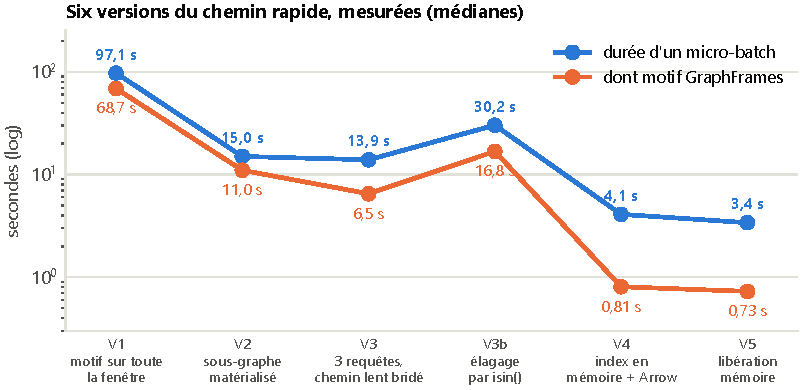
\includegraphics[width=\linewidth]{figures/optimisations.pdf}
\caption[Six versions du chemin rapide]{Durée médiane d'un micro-batch et du motif GraphFrames pour
chaque version du chemin rapide (échelle logarithmique). V1 à 100~tx/s, les suivantes à 50~tx/s.}
\label{fig:optim}
\end{figure}

\begin{table}[htp]
\centering\small
\begin{tabular}{@{}l>{\raggedright\arraybackslash}p{5.8cm}>{\raggedright\arraybackslash}p{6.4cm}@{}}
\toprule
\sffamily\bfseries & \sffamily\bfseries Changement & \sffamily\bfseries Pourquoi ça a (ou n'a pas) marché\\
\midrule
V1 & motif sur tout le graphe glissant & trois auto-jointures de dizaines de milliers d'arêtes à chaque lot\\
V2 & sous-graphe des arêtes candidates \emph{matérialisé} & non matérialisé, il était recalculé pour chaque alias du motif : 86 jobs Spark par lot, contre 6 ensuite\\
V3 & regroupement en 3 requêtes ; chemin lent sur 1--2 partitions, analyses lourdes un passage sur deux, pool FAIR & le chemin lent ne vole plus les cœurs du chemin rapide\\
V3b & élagage des candidats par \fichier{isin()} sur des listes de comptes & \textbf{régression} : chaque valeur littérale coûte un aller-retour Python--JVM\\
V4 & index d'adjacence en mémoire sur le driver ; petits DataFrames construits via Arrow puis \fichier{localCheckpoint} & l'élagage devient une intersection d'ensembles ; Spark connaît la taille des données et choisit des jointures par diffusion\\
V5 & libération explicite des checkpoints locaux ; mémoire native du JVM bornée & latence stable sur 40~minutes (section~\ref{sec:memoire})\\
\bottomrule
\end{tabular}
\caption{Ce qui a changé entre les versions, et pourquoi.}
\label{tab:optim}
\end{table}

\section{Où passe le temps aujourd'hui}
Dans la version finale, le motif GraphFrames ne prend plus que 0,73~s. Le
poste principal est désormais l'écriture dans Delta : chaque micro-batch
valide au moins une transaction Delta (bronze), et jusqu'à quatre quand il
émet une alerte (alertes, sommets et arêtes du sous-graphe) ; chacune coûte
une lecture et une écriture du journal \fichier{\_delta\_log}
(figure~\ref{fig:etapesmb}). C'est ce coût fixe, et non l'analyse de graphe,
qui sépare la plateforme d'une alerte « en sous-seconde ».

\begin{figure}[htp]
\centering
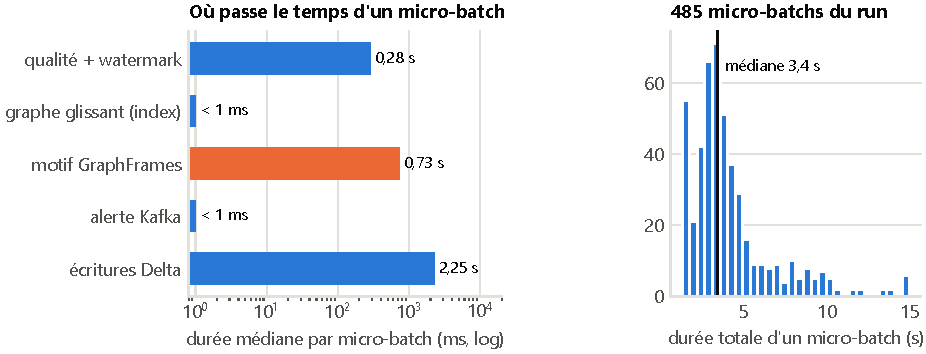
\includegraphics[width=\linewidth]{figures/etapes_microbatch.pdf}
\caption[Décomposition d'un micro-batch]{Décomposition d'un micro-batch pendant le run d'évaluation
(médianes par étape, échelle logarithmique) et distribution de la durée totale.}
\label{fig:etapesmb}
\end{figure}

\section{La mémoire : une fuite invisible}
\label{sec:memoire}
Les premiers runs longs se dégradaient au bout de 20 à 30~minutes. Deux
causes se superposaient. D'abord, \fichier{unpersist()} ne libère pas un
\fichier{localCheckpoint} : ses blocs restent en mémoire jusqu'au ramasse-miettes
périodique de Spark, et le job en accumulait plusieurs centaines (environ
2~Go en 30~minutes). Ensuite, la mémoire \emph{native} du JVM (hors tas Java)
grossissait jusqu'à la limite du conteneur. La version finale libère
explicitement chaque DataFrame matérialisé après usage, déclenche le
nettoyage de Spark toutes les 2~minutes, borne la mémoire directe du JVM
(\fichier{-XX:MaxDirectMemorySize=512m}) et limite le nombre d'arènes de
l'allocateur C (\fichier{MALLOC\_ARENA\_MAX=2}) : la mémoire se stabilise vers
3~Go (figure~\ref{fig:memoire}).

\begin{figure}[htp]
\centering
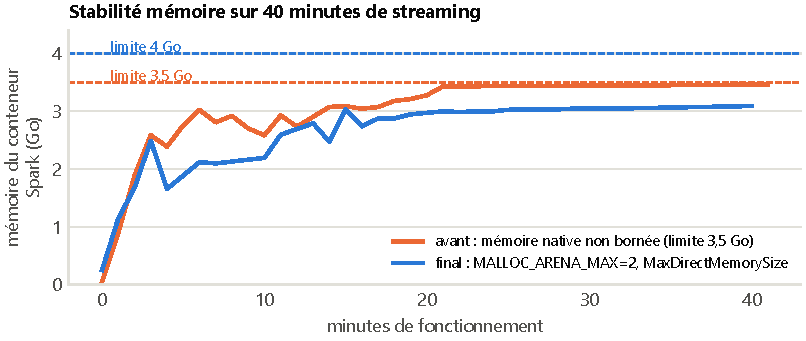
\includegraphics[width=\linewidth]{figures/memoire.pdf}
\caption[Stabilité mémoire]{Mémoire du conteneur Spark (\fichier{docker stats}) au fil de deux runs
de 40~minutes, avant et après la maîtrise de la mémoire native.}
\label{fig:memoire}
\end{figure}

\section{Le chemin lent}
Le chemin lent dispose de 90~secondes par passage. Il en utilise 32 en
médiane (figure~\ref{fig:cheminlentperf}), dont l'essentiel pour PageRank et
la SCC, exécutés un passage sur deux. Ses analyses quotidiennes --- mules,
scatter-gather, pivots --- prennent chacune une à trois secondes.

\begin{figure}[htp]
\centering
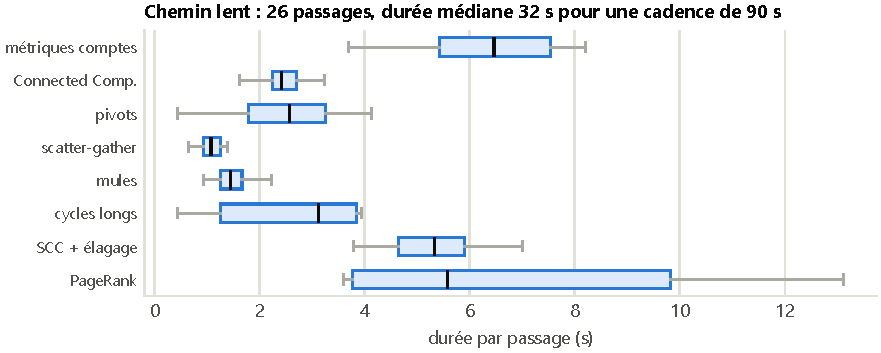
\includegraphics[width=\linewidth]{figures/chemin_lent.pdf}
\caption[Durées du chemin lent]{Durée de chaque analyse du chemin lent sur les passages du run
(boîtes : quartiles ; moustaches : étendue hors valeurs extrêmes).}
\label{fig:cheminlentperf}
\end{figure}

\section{Montée en charge}
Un benchmark injecte successivement 25, 50 et 100~transactions par seconde,
avec un carrousel toutes les 20~secondes, pendant 3~minutes par palier
(figure~\ref{fig:benchmark}). Le débit traité suit la charge et la latence de
détection des carrousels reste autour de 2~secondes : la taille des lots
augmente (50 à 177 lignes en médiane), pas leur durée, car le coût d'un lot
est dominé par ses écritures, pas par le volume.

\begin{figure}[htp]
\centering
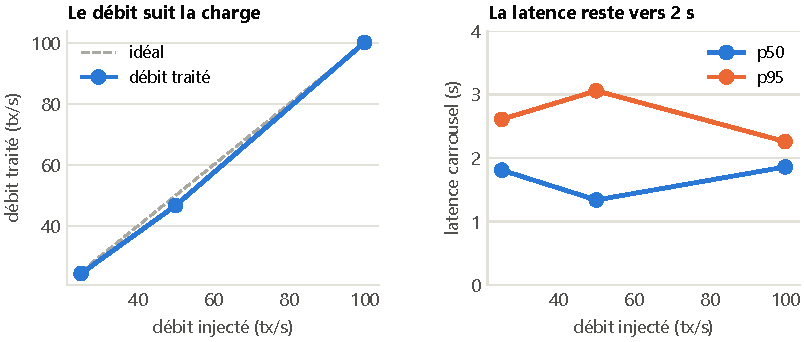
\includegraphics[width=\linewidth]{figures/benchmark.pdf}
\caption[Benchmark de montée en charge]{Benchmark de montée en charge (\fichier{scripts/benchmark.py},
producteur continu arrêté pendant la mesure, 8 carrousels injectés par palier).}
\label{fig:benchmark}
\end{figure}

\section{Leçons retenues}
Le tableau~\ref{tab:lecons} rassemble les règles qu'impose désormais le code,
chacune avec le symptôme mesuré qui l'a fait adopter. Elles sont aussi
consignées dans la documentation du dépôt (\fichier{CLAUDE.md}), pour
qu'aucune ne soit défaite sans nouvelle mesure.

\begin{table}[!htbp]
\centering\small
\begin{tabular}{@{}>{\raggedright\arraybackslash}p{6.2cm}>{\raggedright\arraybackslash}p{8.1cm}@{}}
\toprule
\sffamily\bfseries Leçon & \sffamily\bfseries Symptôme qui l'a révélée\\
\midrule
Matérialiser tout DataFrame réutilisé par un motif & 86 jobs Spark par lot au lieu de 6\\
Construire les petits DataFrames via Arrow, puis \fichier{localCheckpoint} & chaque action relançait des processus Python ($\approx$\,1~s)\\
Ne jamais passer des milliers de littéraux à \fichier{isin()} & régression de V3 à V3b (13,9~s → 30,2~s)\\
\fichier{localCheckpoint} à chaque tour d'une boucle itérative & plan d'exécution doublant à chaque tour, jusqu'à l'erreur mémoire\\
Libérer explicitement les checkpoints locaux & $\approx$\,2~Go perdus en 30~minutes, écritures Delta bloquées\\
Ne pas réactiver le state store RocksDB & arrêt brutal du JVM (« pthread lock: Invalid argument »)\\
\bottomrule
\end{tabular}
\caption{Leçons de performance, et le symptôme mesuré qui a conduit à chacune.}
\label{tab:lecons}
\end{table}

\aretenir{À retenir}{L'analyse de graphe en flux n'est rapide que si l'on ne recalcule jamais ce qui
n'a pas changé : un index incrémental en mémoire pour savoir \emph{où} chercher, GraphFrames pour
\emph{vérifier} sur un tout petit sous-graphe. Le reste est une discipline de mesure : chaque
optimisation a été validée, et une a été annulée, sur des chiffres.}
